% Basic LaTeX template for NE 204 lab report
%defines the type of document you will be using
%Most journals have their own style.
\documentclass[11pt]{article}

%==============================================================================
%%% Everything between the "="'s is the preamble.
%%% Define packages and meta data here

% Common packages
\usepackage{amsmath}    % Expanded math
\usepackage{amssymb}    % Expanded math symbols
\usepackage{graphicx}   % For images
\usepackage[margin=1.0in]{geometry}
%mhchem is beneficial for Nuke Eng.
\usepackage[version=3]{mhchem} % For nuclide formatting
\usepackage{float}

% All images/figures will be stored in the images folder.
% Specify that here so pdflatex knows where to look for images.
\graphicspath{{./images/}}

% Metadata
\title{Experiment 1: Digital Signal Processing for Gamma-Ray Spectroscopy in HPGe}
\author{Christopher Brand}
\date{\today}
%==============================================================================

\begin{document}

% Compile metadata from preamble into a nicely-rendered title section
\maketitle

% The *'s next so section/subsection definitions suppresses numbering
% \section*{Introduction}
\section{Introduction}
\label{sec:intro}
	The goal of this report is to explore some of the various techniques used for digital signal processing. 
This effort utilizes an HPGe detector to explore these techniques through the lens of gamma-ray spectroscopy. 
A trapezoidal shaping filter is implemented and optimized inorder to achieve a final calibrated energy spectrum. 
Through this the effect of ballistic deficit and various contributions to electronic noise are studied to learn about the performance of digital signal processing. 
  


\section{Methods}
\label{sec:meth}
\subsection{Experimental Setup}
A countrate energy spectrum dataset consisting of two sources was gathered with a coaxial high purity germanium detector (HPGE). 
The two sources used were  $^{57}$Co and $^{60}$Co and were used to calibrate the energy spectrum and optimize the filter parameters. The known energies of the calibration peaks are presented below in Table~\ref{tab:CalSrc}.

\begin{table}[H]
        \begin{center}
                \begin{tabular}{l|r}
                        \textbf{Source} & \textbf{Energy (keV)}\\
                        \hline
                        $^{57}$Co      &       136.47    \\
                        $^{60}$Co      &       1173.22, 1332.49   \\
                \end{tabular}
                \caption{Source Isotopes and Corresponding Gamma-ray energies}
                \label{tab:CalSrc}
        \end{center}
\end{table}

Additionally, data was collected by generating a pulse from a generator. This simulated data was used to optimize the filter parameter and study noise from the system. 
All of this data was collected through a digitization system from Struck Innovative Systems (SIS), SIS3302 module. Inorder to gather this data and parse it from the module,
custom c++ based software was provided and then modified for our endeavor. The data parsed into the standard .h5 file format. 

\subsection{Trapizoidal Filter Implemination}
	
	A script with a trapizoidal filter  was created using python 3.5, based off of the work done by V. Jordanov et. al.\cite{jordanov1994digital}. In addition an input spectrum, there are two parameters needed,
	the rise time, k, of the trapizoid and the gap time,m or the trapizoid. The gap time was found by iterating passing a number of values of m through the script and finding the energy resolution of one of the  $^{60}$Co peaks. From this a energy resolution vs rise time graph was plotted and a minimized value for m was attempted to be found. An attempt was done to find the rise time, k, in much the same manner, however, the simulated pulse was used in this case so as to be able to evaluate the contributions of the various electronic noise components. 

\subsection{Energy Calibration}

        The gamma-ray spectrum is approximated as being composed of a global non-linear background with guassian peaks due to the impingment of high branching ratio gamma-ray lines from radioactive decay.\cite{Knoll} The peaks are fitted by a Gaussian of the form:

\begin{equation}
G(x; A,\mu, \sigma) = A\exp\bigg(-\frac{(x-\mu)^2}{2\sigma^2}\bigg)
\end{equation}

Where x is the data, A is the amplitude, mu is the mean, and sigma is the standard deviation. Additionally, the data was then fit to a linear model as in lab0.  





\section{Results}
\label{sec:res}
\subsection{Trapizod Filter Parameters}
The opimization method used as oulined in Section~\ref{sec:meth}, resulted in the following two graphs:

\begin{figure}[!htb]
\centering
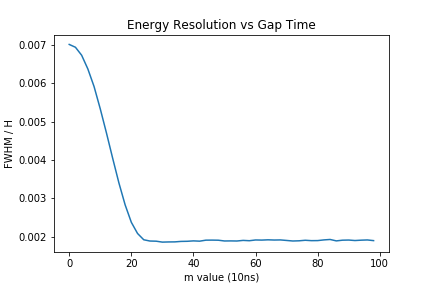
\includegraphics[width=0.7\linewidth]{images/RvsM.png}
\caption{ gap time, m, vs Energy Resolution as compared to the ${60}$Co's 1332 keV peak.}
\label{fig:MvsER}
\end{figure}


\begin{figure}[!htb]
\centering
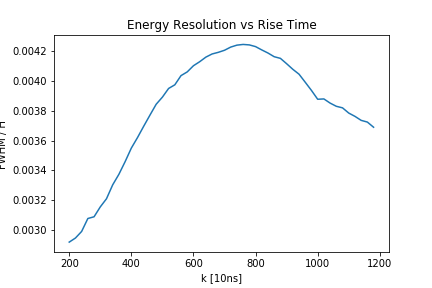
\includegraphics[width=0.75\linewidth]{images/RvsK_main.png}
\caption{ rise time, k, vs Energy Resolution as compared to the simulated pulse peak.}
\label{fig:kvsER}
\end{figure}


While Figure \ref{fig:MvsER} looks acceptable, Figure \ref{fig:kvsER} has the appearance of being inverted. This is disscused further in Section ~\ref{sec:dis}. 
The optimized m value was 30 +/-2 and the used k value was 740 +/- 20.
Additionally, the decay time was found to be 5810.2.

\subsection{Data Signals}
The following are five examples of signals from the 57Co data set before and after being put through the filter:

\begin{figure}[!htb]
\centering
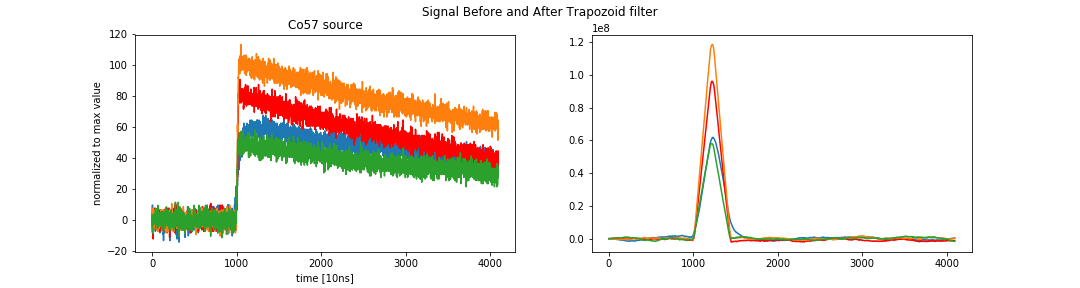
\includegraphics[width=1.0\linewidth]{images/5signals_3.png}
\caption{ Left: Raw Data signals from the SIS3302. Right: Same signals after going through the optimized trapizoidal filter.}
\label{fig:signals}
\end{figure}


\subsection{Energy Spectrum}
The following are the final energy spectra with the energy calibration done:

\begin{figure}[!htb]
\centering
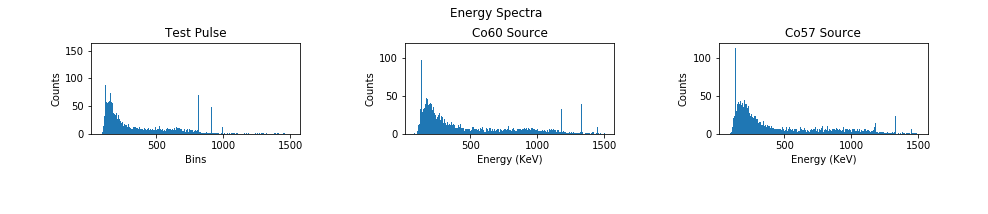
\includegraphics[width=1.0\linewidth]{images/BinnedData_3_energy.png}
\caption{ From left to right: Test Pulse Spectrum, Co57 Spectrum, Co60 Spectrum}
\label{fig:EngSpec}
\end{figure}




A discovered issue with these data set was the intense background contribution from other sources. This is discussed further in Section ~\ref{sec:dis}.


The peak selection and fitting procedure outlined in Section~\ref{sec:meth}, resulted in a linear energy calibration of the form
\begin{equation}
E = 0.1731*Bin + 82.76
\end{equation}


The energy resolution of the 3 peaks are as follows:


\begin{table}[H]
        \begin{center}
                \begin{tabular}{l|r}
                        \textbf{Peaks} & \textbf{Energy Resolution}\\
                        \hline
                        136.47      &       0.27     \\
                        1173.22     &       0.0104   \\
			1332.49     &       0.0078   \\ 
                \end{tabular}
                \caption{Energy Resolution for one 57Co peak and two 60Co peaks}
                \label{tab:CalSrc}
        \end{center}
\end{table}


\section{Discussion}
\label{sec:dis}
A major concern with digital processing of signals is ballistic deficit. ballistic deficit is the different in amplitude between the shaped pulse (after it leaves the amplifier) 
and the original pulse. This difference arises when the rise time of the original pulse is on the order of the shaping time in the amplifier, meaning that pulses will have smaller amplitudes,
providing us with the incorrect energy information. These pulses can be corrected to an extent by sending the pulse through a trapizoidal filter as seen in Figure 3 of Section 3. 
The flat top of the trapizoid, also known as the gap time, m, stabalizes the amplitudes so that they do not suffer from ballisti deficit. This can be seen in Figure 1 of Section 3, 
where a number of m where compared to the energy resolution of a single peak. At low gap time (a triangle filter), the peak has low energy resolution and the peak has been broadend
due to ballistic deficit. However, as we increase the gap time, the peak becomes more precise, because of the reduction of the ballistic deficit until it bottems out at ~300 +/-20 [ns]. After this,
the gap time is no long able to reduce the ballistic deficit and so greater gap times are not useful. It should be noted that in this case, the error is entirly due to the large step size 
choosen to minimize the gap time (steps of 20ns). This was done merely to save on time as the code takes time to run. Other sources of error, such as electronic noise and fit errors are negligible
compared to the uncertainty due to the step size. 
\linebreak
\linebreak
In order to study the contributions of the various electronic noise components, the rise time,k, of the trapizoid was varied while looking at a simulated pulse from a pulse generator. Doing this
assures us that a majority of the noise that is seen comes from the internal electronics rather then from background or other sources. The results are shown in Figure 2 from Section 3. 
This plot is not correct. Unfortuantly I was unable to figure out the problem in my code, however, inverting this graph produces a graph that looks like what I am suppose to get. I am going
to assume that the inverse of this graph is correct for the purposes of discussing the various contributions to noise. This figure is shaped like a parabola because of the large contributions 
due to series (voltage) noise and parallel (current) noise. Low rise times results in high contributions from series noise such as thermal (electron velocity changes that create voltage noise) 
 and Johnson (noise from resistors changing the voltage  effects. At high rise times the noise
again increases due to larger and larger contributions from parallel noise such as shot noise (flucuations of the current due to changes in kinetic energy of the electrons). The supposed graph
would indicate that for all k series and parallel noise are the primary contribitor since any 1/f noise would result in a flat (ish) line. 1/f or flicker noise is the fundimental alterations 
that exsit in all thing in nature. The optimal k found is 7400 +/- 200 [ns]. It should be noted that the error is entirly due to the large step size 
choosen to minimize the gap time (steps of 20ns). This was done merely to save on time as the code takes time to run.  
\linebreak
\linebreak
One draw back to this filtering method is that it breaks down at higher count rates. So it is recommended that this method be used only for low count rates. That being said, I would recommend 
taking more data then I took for this lab. The lack of counts I had in my spectrum made it difficult to find peaks. Additionally, greater care should have been taken in isolating the sources from 
background. After analysing the data it can be seen in Figure 4 Section 3, that additional peaks from other sources appear. This made the analysis more uncertain, as there is uncertainty to what 
excalty these peaks were. Additionally, the lower energy peaks in the 57Co could not be seen. 


% Bibliography
\bibliographystyle{plain}
% Refers to a bibtex file in the current dir named "references.bib"
\bibliography{references}

\end{document}
